\documentclass{article}

\usepackage{amssymb}
\usepackage[intlimits]{amsmath}
\usepackage{graphicx}
\usepackage{verbatim}
\usepackage{empheq}
\usepackage{bbm}
\usepackage{bm}
\usepackage{fullpage}
\usepackage{mathtools}
\usepackage{caption}
\usepackage{subcaption}
\usepackage{algorithm}
\usepackage{algpseudocode}
\usepackage{courier}

\usepackage{hyperref}
\hypersetup{
    colorlinks,
    citecolor=blue,
    filecolor=blue,
    linkcolor=blue,
    urlcolor=blue
}

\newcommand{\Prob}[1]{\ensuremath{\mathbb{P}\left[#1\right]}}
\newcommand{\CondP}[2]{\ensuremath{\mathbb{P}\left[#1|#2\right]}}
\newcommand{\Exp}[1]{\ensuremath{\mathbb{E}\left[#1\right]}}
\newcommand{\Var}[1]{\ensuremath{\text{Var}\left[#1\right]}}
\newcommand{\Std}[1]{\ensuremath{\text{Std}\left[#1\right]}}
\newcommand{\CondE}[2]{\ensuremath{\mathbb{E}\left[#1|#2\right]}}
\newcommand{\inner}[2]{\ensuremath{\left<#1,#2\right>}}
\newcommand*\widefbox[1]{\fbox{\hspace{2em}#1\hspace{2em}}}
\renewcommand{\(}{\left(}
\renewcommand{\)}{\right)}

\newcommand{\txtmathbf}[1]{\ensuremath{\text{\textbf{#1}}}}

\newtheorem{theorem}{Theorem}
\newtheorem{lemma}[theorem]{Lemma}
\newtheorem{claim}{Claim}
\newenvironment{proof}{{\bf Proof:}}{\hfill\rule{2mm}{2mm}}

\newtheorem{definition}{Definition}
\let\olddefinition\definition
\renewcommand{\definition}{\olddefinition\normalfont}

\DeclareMathOperator*{\argmin}{argmin}
\DeclareMathOperator*{\argmax}{argmax}

\graphicspath{{plots/}}

\title{CS155 Kaggle Project Report}
\author{Daniel Chao\thanks{Team partners listed alphabetically.} \and Jae Hong Kim\footnotemark[1]}
\date{\today} 

\begin{document}

\maketitle 
\tableofcontents 

\section{Overview}
The objective of CS155 Kaggle project was to classify the annual reports by publicly traded companies to the U.S. Securities and Exchange Commission on whether it was submitted during the Great Recession from Dec. 2007 to Jun. 2009 or not.  The data is given to us in two different formats, which will be discussed in more detail in Section~\ref{sec:models}, and consists of 4000 documents and their labels for the training data set and 9868 documents for the test data set where each document is represented as a point in a 500 dimensional feature space.  In addition, we are given public leaderboard during the competition to which we can submit our predictions and receive the feedback based on $40\%$ of the test set.  Although the public leaderboard was a useful tool to gauge our current status, we tried not to rely on it too much as we did not want to overfit on that specific test set.  

Our approach to the project was to use ensemble selection \cite{caruana04}, which requires generation of a large model library and implementation of the ensemble assembly.  Within our team, Jae focused on generating the model library using \texttt{scikit-learn} implementations and Daniel focused on ensemble selection which did not use any pre-existing packages.  Our team handle on the Kaggle site was "DrOPitlikEitshot".

\section{Generating the model library} \label{sec:models}
In this section, we present brief descriptions of the approximately 2000 models that make up our model library.  Ensemble selection requires overproducing a large number of classifiers for various learning algorithms.  Each model consists of a unique combination of input processing and an instantiation of a learning algorithm that is used to transform and fit the training data set and predict the labels of the test data set.  All input processing and learning algorithms used were \texttt{scikit-learn} implementations.  

  \subsection{Input processing}

  \begin{itemize}
    \item \textbf{TF-IDF}: Term frequency-inverse document frequency, or tf-idf, is a feature representation of a collection of documents, or a corpus. By using a bag of words as the feature space, we can project a document in the corpus onto a numerical vector.  An example is a simple word count normalized by the total number of words, which suffers from inherent bias towards lesser meaningful words such as `the' and `is'.  Tf-idf attempts to overcome this by weighting the term frequency within a document by the overall term frequency across the entire corpus.  For this project, we are given both word count and tf-idf representations of the data.  Due to time constraints, we chose to make use of only the tf-idf data, which we deemed to be a more sensible representation for relative importance of keywords.

    \item \textbf{Centering and Scaling}: Centering is a transformation that subtracts the mean of the data set as to make the data have zero mean.  This removes any bias a feature might have from the way it was collected. Whereas centering is a uniquely defined procedure, scaling the data can be done in different ways. For our library, we employ two scaling methods, one is normalizing the data to unit variance (i.e. dividing each feature by its standard deviation) and the other is scaling each feature to be within a specified range (e.g. [-1, 1]).     

    \item \textbf{Feature Selection}: The training data set contains 4000 points, where each point is represented by a point in a 500-dimensional feature space.  We were concerned that the 500-demensional model would overfit the data, so we tried reducing the number of features using principal component analysis (PCA) and L1-based feature selection.

PCA can be used to rank a feature based on amount of information it carries, which is captured by its variance; the overall loss of information by reducing the feature space can be described by the reconstruction error $E_{\text{r}} = \|\mathbf{X}-\mathbf{X}_r\|^2$, or the Frobenius norm of difference between the originial design matrix and the reduced design matrix reconstructed in the originial feature space. Figure~\ref{fig:top-k} shows the reconstruction error as a function of the number of components kept for our training data set.  As we can see, the error decreases rapidly when the first few features are kept as they contain the most information.  For building the model library, we tried both keeping all features and reducing the number of features to 200, which corresponded to about $15\%$ reconstruction error.   

      \begin{figure}
	\centering
	  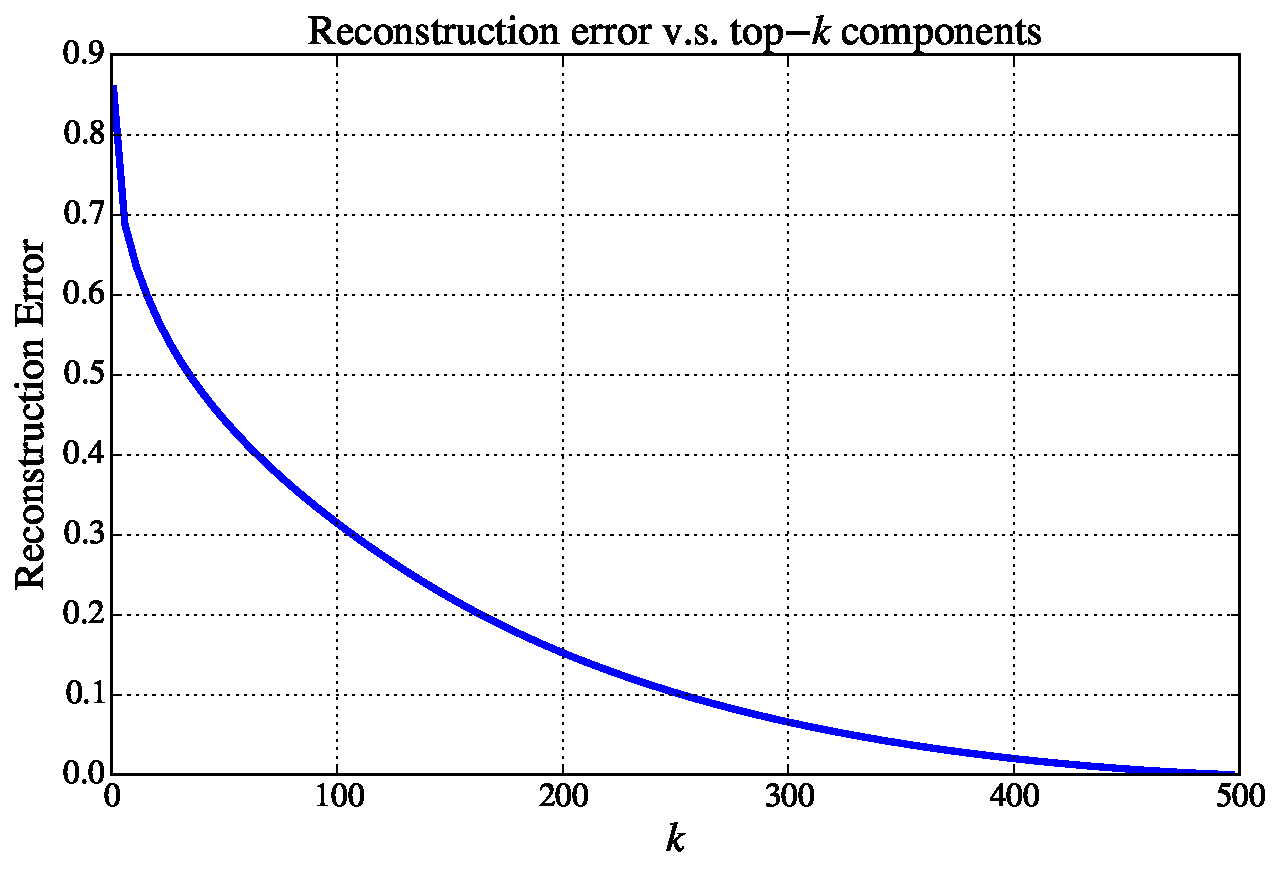
\includegraphics[width=0.4\textwidth]{top-k_PCA}
	\caption{}
	\label{fig:top-k}
      \end{figure}

L1-based feature selection uses the fact that linear models regularized by the L1-norm results in sparse solutions, resulting in another way to remove less important features.  The amount of reduction of feature space is control by the regularization parameter $C$ in the objective function.  For certain learners, we applied L1-based feature reduction using various values of $C:\{0.001, 0.01, 0.1\}$.

    \item \textbf{Whitening}: Whitening is a transformation that decorrelates a set of data.  Practically speaking, this is accomplish by transforming the covariance matrix of the data into an identity matrix (i.e. features are uncorrelated with unit variance).  It is clear that whitening, if done at all, should be done after feature selection.  As similar to feature selection, we explored the both options of learning on whitened and unwhitened data.   
  \end{itemize}
  
  \subsection{Learning algorithms}
  As most of the learning algorithms used in this project were discussed during class lectures, this section mostly aims to describe our approach to exploring the parameter space grid of each learner, where the reasonable starting values for the parameters were taken from the work by Niculescu-Mizil et al. \cite{KDD}.

  \begin{itemize}
    \item \textbf{Logistic Regression}: Logistic regression is a linear classification model that seeks to maximize the likelihood, or equivalently minimize the log loss.  In addition, the model can be regularized using either L1 or L2 penalty.  More concretely, logistic regression can be represented as the following optimization problem:
      \begin{equation} \label{eq:logreg}
	\argmin_{\mathbf{w}} \frac{1}{2}\|\mathbf{w}\|^2 + C\sum_i\log\left(\exp\left(-y_i\mathbf{x}_i^T\mathbf{w}\right)+1\right),
      \end{equation}
      where $\mathbf{x}_i$ and $y_i$ are the \emph{i}-th data point and its label, $\mathbf{w}$ is the vector of weights, and $C$ is the regularization parameter for the L1- or L2-norm of the weights.

      We generated the models for the library by first centering and normalizing the data, then varying the number of features used $\{200, 500\}$, the type of penalty used, $C:\{10^{-5}, 10^{-4}, 10^{-3}, 10^{-2}, \allowbreak 10^{-1}, 1, 10^{1}, 10^{2}\}$, whether to include a constant bias term in the log loss, and whether to balance the data to account for the fact that the training data consisted of $17\%$ of data with label $1$.  The data balancing was done either automatically based on the frequency of class labels or manually by weighting the label class $0/1$ by $1/3$, respectively. 

    \item \textbf{Support Vector Machine}: Support vector machine is a max-margin classifier, where the model tries to linearly separate the data while maximizing the distance between the separating hyperplane and the closest data points, which is the margin. In most cases, the data is not linearly separable due to noise, thus classifiers called soft-margin SVM's allow violation of the margin.  One forumation of soft-margin SVM is:
      \begin{equation} \label{eq:svm}
	\begin{split}
	  &\argmin_{\mathbf{w}} \frac{1}{2}\|\mathbf{w}\|^2 + C\sum_i\xi_i \\
	  &\text{subject to } y_i \left(\mathbf{w}^T \phi(\mathbf{x}_i)+b\right)\ge 1-\xi_i \text{ and } \xi_i \ge 0\;\forall i,
	\end{split}
      \end{equation}
      where $\xi_i$ is the the parameter representing the amount of violation allowed for \emph{i}-th data point and $\phi^T\phi$ is the kernel function which transforms the data into a higher dimensional represenation. 

      We generated many SVM models by first preprocessing the data to be scaled within the range [-1, 1] and then either reducing feature dimensions to 200 and whitening or not reducing and whitening.  The kernel functions used are: radial basis functions (RBF) for which we vary its width parameter $\gamma:\{0.001, 0.005, 0.01, 0.05, 0.1, 0.5, 1., 2.\}$, polynomials functions of degrees 2, 3, and 5, and a linear function. For all kernels, we vary the regularization parameter $C$ from $10^{-7}$ to $1000$ in factors of $10$.    

      After scoring the first set of models using cross validation, which will be described in Section~\ref{sec:ensemble} , we trained more SVM with RBF kernel with finer grid of $\gamma$ and $C$, and also balancing the data.

    \item \textbf{Boosted Decision Trees}: Boosting refers to iteratively learning a data set using a collection of "weak" learners, where a weak learner is a learned model with low predictive power.  This method takes adventage of the low variance of weak learners, while the inherently high bias of the weak learners are reduced by the ensemble nature of boosting.  The algorithm used for boosting this set of decision trees for classification is AdaBoost, and we vary the depth of the base classifier $\{1, 2, 3, 4, 5, 7, 10, 20\}$, number of rounds of boosting among 30 numbers between 1 and 1200, and the learning rate $\{0.7, 1\}$.  The learning rate acts as a regularizor for the model and may result in for better generalization.  The criterion used for splitting for the base classifier is the gini criterion. 

      We processed the inputs using centering and normalization, and then for some models reducing the feature space using L1-based feature selection using $C:\{10^{-3}, 10^{-2}, 10^{-1}\}$, where smaller value of $C$ implies larger reduction. Lastly, we also try balancing the data for some models.

    \item \textbf{Gradient Tree Boosting}: Gradient tree boosting is another method of boosting trees similar to AdaBoost.  Whereas AdaBoost is used only for classification, gradient boosting can be used for both regression and classification.  Although the concepts are similar, the differences in the algorithm might result is different generalization, thus we decided to include some models traine using gradient tree boosting.

      We generate different models by varying the number of rounds of boosting, the maximum depth of the base tree classifier, and the learning rate in a similar way as we did for the boosted decision trees. 

    \item \textbf{Random Forest}: In constrast to the boosting methods, random forest seeks to take adventage of the low bias and high predictive power of deeper and more complex decision trees.  As complex trees are prone to overfitting, random forest creates an ensemble of such trees where each tree is trained using different subsets of the data (bagging) and features. Bagging, or bootstrap aggregation, reduces the variance of the base classifiers and is not limited only to decision trees.    

      We generated various instantiations of random forest by varying the input processing, from centering and normalizing to feature selection using Lasso.  We tried learning on the raw unprocessed data, but the performance of those random forests were mediocre at best.  In addition, we vary the number of trees in the forest $\{256, 512, 1024\}$, the number of features to be considered for each split between 1 and 500, and the criterion for splitting between gini and information gain.  We also try balancing the data for some models.   
  \end{itemize}

\section{Ensemble selection (Dan)} \label{sec:ensemble}
Describe how ensemble selection was performed. Also describe methods for regularizing the ensemble. 

\section{Conclusion **add anything you want to improve**}
In the end, the ensembles with high number of rounds of bagging simply took too long to run, so our final submissions were not as optimal as we planned.  For building the model library, it would have been better to explore different learning algorithms including neural network and unsupervised learning such as k-Nearest Neighbors, and to have a more systematic way of searching for well-performing regions in the parameter grid.  Furthermore, we didn't pursue too deeply into effciently training the data such as taking adventage of the sparsity.  

\begin{thebibliography}{99}
\bibitem{caruana04}
  R. Caruana and A. Niculescu-Mizil.
  (2006).
  Ensemble selection from libraries of models.
  \emph{ICML '04}.
\bibitem{KDD}
  A. Niculescu-Mizil \emph{et al}.
  (2009).
  Winning the KKD Cup Orange Challenge with Ensemble Selection.
  \emph{KDD Cup 2009}.

\end{thebibliography}

\end{document}
